%% Преамбула TeX-файла

% 1. Стиль и язык
\documentclass[utf8x]{G7-32} % Стиль (по умолчанию будет 14pt)
\usepackage[T2A]{fontenc}
\usepackage[russian]{babel}
% Остальные стандартные настройки убраны в preamble.inc.tex.
\sloppy

% Настройки стиля ГОСТ 7-32
% Для начала определяем, хотим мы или нет, чтобы рисунки и таблицы нумеровались в пределах раздела, или нам нужна сквозная нумерация.
\EqInChapter % формулы будут нумероваться в пределах раздела
\TableInChapter % таблицы будут нумероваться в пределах раздела
\PicInChapter % рисунки будут нумероваться в пределах раздела

% Добавляем гипертекстовое оглавление в PDF
\usepackage[
bookmarks=true, colorlinks=true, unicode=true,
urlcolor=black,linkcolor=black, anchorcolor=black,
citecolor=black, menucolor=black, filecolor=black,
]{hyperref}

% Изменение начертания шрифта --- после чего выглядит таймсоподобно.
% apt-get install scalable-cyrfonts-tex

\IfFileExists{cyrtimes.sty}
    {
        \usepackage{cyrtimespatched}
    }
    {
        % А если Times нету, то будет CM...
    }

\usepackage{graphicx}   % Пакет для включения рисунков

% С такими оно полями оно работает по-умолчанию:
% \RequirePackage[left=20mm,right=10mm,top=20mm,bottom=20mm,headsep=0pt]{geometry}
% Если вас тошнит от поля в 10мм --- увеличивайте до 20-ти, ну и про переплёт не забывайте:
\geometry{right=20mm}
\geometry{left=30mm}


% Пакет Tikz
\usepackage{tikz}
\usetikzlibrary{arrows,positioning,shadows}

% Произвольная нумерация списков.
\usepackage{enumerate}

% ячейки в несколько строчек
\usepackage{multirow}

% itemize внутри tabular
\usepackage{paralist,array}


% Настройки листингов.
% 8 Листинги

\usepackage{listings}

% Значения по умолчанию
\lstset{
  basicstyle= \footnotesize,
  breakatwhitespace=true,% разрыв строк только на whitespacce
  breaklines=true,       % переносить длинные строки
%   captionpos=b,          % подписи снизу -- вроде не надо
  inputencoding=koi8-r,
  numbers=left,          % нумерация слева
  numberstyle=\footnotesize,
  showspaces=false,      % показывать пробелы подчеркиваниями -- идиотизм 70-х годов
  showstringspaces=false,
  showtabs=false,        % и табы тоже
  stepnumber=1,
  tabsize=4,              % кому нужны табы по 8 символов?
  frame=single
}

% Стиль для псевдокода: строчки обычно короткие, поэтому размер шрифта побольше
\lstdefinestyle{pseudocode}{
  basicstyle=\small,
  keywordstyle=\color{black}\bfseries\underbar,
  language=Pseudocode,
  numberstyle=\footnotesize,
  commentstyle=\footnotesize\it
}

% Стиль для обычного кода: маленький шрифт
\lstdefinestyle{realcode}{
  basicstyle=\scriptsize,
  numberstyle=\footnotesize
}

% Стиль для коротких кусков обычного кода: средний шрифт
\lstdefinestyle{simplecode}{
  basicstyle=\footnotesize,
  numberstyle=\footnotesize
}

% Стиль для BNF
\lstdefinestyle{grammar}{
  basicstyle=\footnotesize,
  numberstyle=\footnotesize,
  stringstyle=\bfseries\ttfamily,
  language=BNF
}

% Определим свой язык для написания псевдокодов на основе Python
\lstdefinelanguage[]{Pseudocode}[]{Python}{
  morekeywords={each,empty,wait,do},% ключевые слова добавлять сюда
  morecomment=[s]{\{}{\}},% комменты {а-ля Pascal} смотрятся нагляднее
  literate=% а сюда добавлять операторы, которые хотите отображать как мат. символы
    {->}{\ensuremath{$\rightarrow$}~}2%
    {<-}{\ensuremath{$\leftarrow$}~}2%
    {:=}{\ensuremath{$\leftarrow$}~}2%
    {<--}{\ensuremath{$\Longleftarrow$}~}2%
}[keywords,comments]

% Свой язык для задания грамматик в BNF
\lstdefinelanguage[]{BNF}[]{}{
  morekeywords={},
  morecomment=[s]{@}{@},
  morestring=[b]",%
  literate=%
    {->}{\ensuremath{$\rightarrow$}~}2%
    {*}{\ensuremath{$^*$}~}2%
    {+}{\ensuremath{$^+$}~}2%
    {|}{\ensuremath{$|$}~}2%
}[keywords,comments,strings]

% Подписи к листингам на русском языке.
\renewcommand\lstlistingname{\cyr\CYRL\cyri\cyrs\cyrt\cyri\cyrn\cyrg}
\renewcommand\lstlistlistingname{\cyr\CYRL\cyri\cyrs\cyrt\cyri\cyrn\cyrg\cyri}


% Полезные макросы листингов.
% Любимые команды

\newtheorem{theorem}{Теорема}
\newtheorem{definition}{Определение}

\newcommand{\Code}[1]{\textbf{#1}}


\newcommand{\myImage}[3]{
\begin{figure}[!ht]
    \centering
    \includegraphics[width=\textwidth]{figures/#2}
    \caption{#1}
    \label{#3}
\end{figure}
}


\begin{document}

\pagestyle{empty}
\begin{center}
    Министерство образования и науки Российской Федерации\\
    ФГАОУ ВПО  «УрФУ имени первого Президента России Б. Н. Ельцина»\\
    Институт радиоэлектроники и информационных технологий - РтФ\\
    Департамент информационных технологий и автоматики
    \par
    \vspace{4.5cm}
    \Large{
      Иммитационное моделирование в  системе Bizagi Proces Modeler

      \par
      \vspace{0.5cm}

      ОТЧЕТ\\
      по лабораторной работе
    }

    \vspace{4cm}
    {
      Преподаватель: \hfill Клебанов Борис Исаевич
    }
    \par
    {
      Студент: \hfill Сухоплюев Илья Владимирович
    }
    \par
    {
      Группа: \hfill РИ-440001
    }

    \par
    \vspace{3.5cm}
    Екатеринбург\\
    2017
\end{center}


\frontmatter % выключает нумерацию ВСЕГО; здесь начинаются ненумерованные главы: реферат, введение, глоссарий, сокращения и прочее.

% Команды \breakingbeforechapters и \nonbreakingbeforechapters
% управляют разрывом страницы перед главами.
% По-умолчанию страница разрывается.

% \nobreakingbeforechapters
% \breakingbeforechapters

\pagestyle{plain}

\tableofcontents


\Introduction

Целью работы является создание всякой всячины. Для достижения поставленной цели необходимо решить следующие задачи:

\begin{itemize}
\item проанализировать существующую всячину;
\item спроектировать свою, новую всячину;
\item изготовить всякую всячину;
\item проверить её работоспособность.
\end{itemize}

Вот так-то. А этот абзац вставлен для визуальной оценки отступа от перечня до следующего абзаца.

\mainmatter % это включает нумерацию глав и секций в документе ниже

\chapter{Установка Bizagi Studio}

Первым этапом в ознакомлении с BPM-системами, встающим при начале разработки,
является установка соответствующих инструментов. В нашем случае, мы
можем скачать устоновочную программу с официального сайта
\textit{Bizagi}(\url{https://www.bizagi.com/}) в ознакомительных целях.

Сама установка программных компонент является тривиальной последовательнустью
действий, выполняемых с помощью мастера установки. Единственной проблемой,
которая может возникнуть -- это специальные требования к СУБД, которые
хорошо описаны в документации к Bizagi Studio
\cite[SQL Server requisites]{sql-requisites}: потребуется установить базу
данных \textit{MS SQL EXPRESS} (версии описанной в документации), а так же
сустему управления этой базой данных (\textit{MS SQL Managenment Studio}),
чтобы провести необходимую предварительныю настройку (разрешение подключения к БД
с помощью логина\\пароля и создание учетной записи администратора для Bizagi Studio).

В дальнейшем нам достаточно лишь запустить Bizagi Studio (Рис. \ref{20-bizagi-studio}),
задать имя у нового проекта (Рис. \ref{20-create-project}) и описать подключение
к настроенной базе данных (Рис. \ref{20-database}). И если все указано верно,
мы увидим карусель разработки web-приложения (Рис. \ref{20-carrousel}).

\myImage{Приветствующий экран Bizagi Studio}{20-bizagi-studio}{20-bizagi-studio}
\myImage{Создание нового проекта}{20-create-project}{20-create-project}
\myImage{Указание настроек подключения к БД}{20-database}{20-database}
\myImage{Карусель разработки созданного проекта}{20-carrousel}{20-carrousel}

\chapter{Импорт BPMN-схемы услуги}

Теперь перейдем к первому этапу проектирования нашего приложения
для услуги Совет да любовь - описания этого бизнес процесса в виде
графического представления в специальной нотации (BPMN).

В нашем случае, ознокомление с данной натацией было проведено в предудущей
лабораторной работе, и нам достаточно просто импортировать готовую схему
нашего процесса в проект (Рис. \ref{30-import}).

\myImage{Выбираем пункт <<Import process>>,
чтобы добавить готовую BPMN-диаграмму}{30-import}{30-import}

После чего мы можем в открывшемся окне \textit{Bizagi Modeler} подкорректоровать
при необходимости нашу схему (Рис \ref{30-description}). На схеме как раз
отображаются основные моменты проведения услуги: гражданин РФ, имеющий быть
честь предоставленный к награде <<Совет да любовь>>, может подать заявление
в многофункциональный центр (МФЦ), после чего в ходе некоторых проверок
(уточнение сведений о судимости в Информационном центре (ИЦ) и проверке соблюдения
прав детей заявителя) Министерство социальной политики заполняет наградной лист
и формулирует предложения о нагрождении, после чего передает все это в Правительство.

\begin{sidewaysfigure}
    \centering
    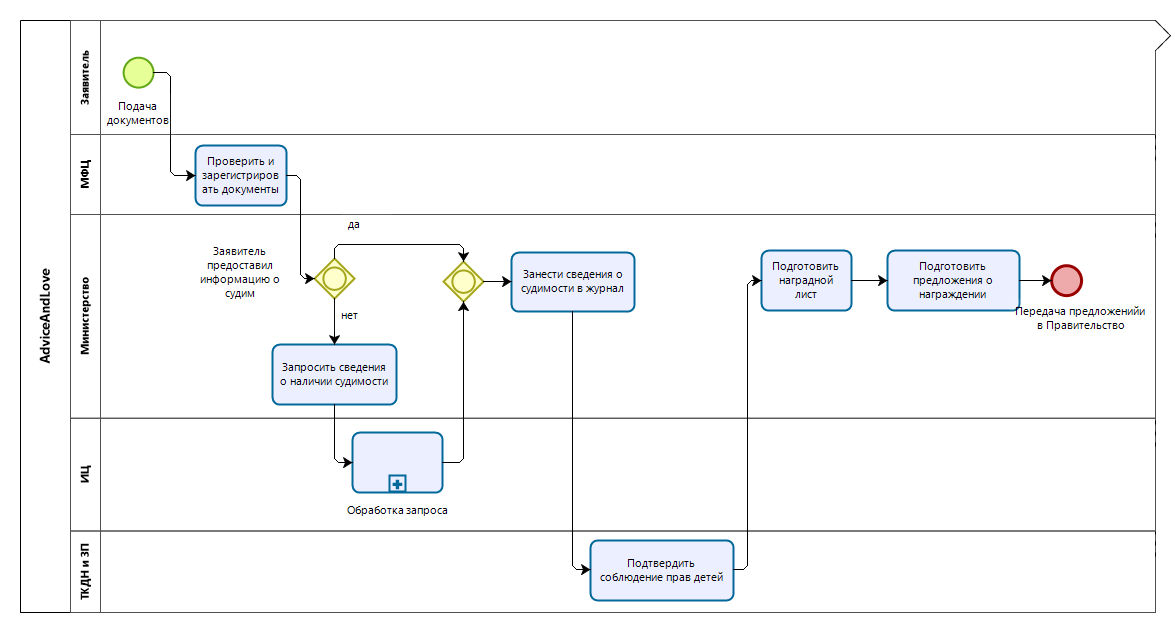
\includegraphics[width=\textwidth]{figures/30-BPMN}
    \caption{Улуга <<Совет да любовь>> в нотации BPMN}
    \label{30-description}
\end{sidewaysfigure}
\chapter{Разработка инфологической модели для БП}

Описав бизнес процесс можно перейти к следующему этаапу. Повернув карусель разработки
вправо, мы перейдем к пункту <<Model data>>. В нем можно перйти к описанию
диограмм сущностей для баз данных. Чтобы добавить основную информацию к нашему процессу,
выберем пункт <<Properties>> в выпадающем меню (Рис. \ref{40-properties}).

\myImage{Выбираем пункт <<properties>>}{40-properties}{40-properties}
\clearpage

Там, мы можем подкорректировать видимое название у нашего рпоцесса, а также в
аттрибутах мы опишем основные данные, которые будут заполняться при работе WEB-приложения:
Имя и Фамилия заявителя, контактный телефон для связи, а также поля для
сканов всех необходимых документов участвующих в нашей услуге.

\myImage{Заполняем аттрибуты нашей услуги -- все необходимые документы}{40-attributes}{40-attributes}

\chapter{Разработка пользовательского интерфейса}

Описав основные документы, которые необходимо заполнить при предоставлении услуги,
нам требуется описать, как они будут заполнятся.

К счастью, в Bizagi Studio есть полноценный редактор форм, с помощь которого
можно создать необходимые формы в несколько кликов мыши.

\myImage{Перейдя в <<Define Forms>>, нам нужно выбрать для какого
действия нужно создать формы (помечены восклицательным знаком)}{50-add-form}{50-add-form}
\myImage{Перетаскивая аттрибуты данных на форму,
можем легко сформировать панель для регистрации инструментов
(Красным подсвечены поля обязательные для заполнения на данном этапе)
}{50-register-form}{50-register-form}
\myImage{Отправка запроса в ИЦ - не может быть автоматизирвоана по внешним причинам,
поэтому просто дадим исполнителю необходимую информацию и добавим подтверждение
об отправке заявления в ИЦ}{50-request}{50-request}

\myImage{Внесение сведений о судимости в модель.
На этом этапе остальные поля уже не меняются}{50-journal}{50-journal}
\begin{figure}[!ht]
    \centering
    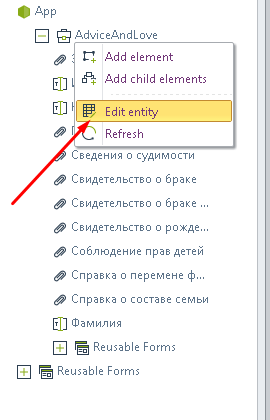
\includegraphics[width=0.5\textwidth]{figures/50-edit}
    \caption{При необходимости, можно отредактировать модель прямо в редакторе форм}
    \label{50-edit}
\end{figure}
\chapter{Настройка бизнес-правил шлюзов}

Для целостной работы форм вместе, нем осталось описать логику работы
шлюза в зависимости от наличия свидетельства о судимости на предыдущем этапе
работы.


\myImage{Выбираем нужный шлюз, а после ветку для которой бедм задавать условие}{60-choose}{60-choose}
\myImage{Переход по ветку <<да>> будет при выполнении условия}{60-yes}{60-yes}
\myImage{Описание условия перехода: Сведения о судимости не пусты (not null)}{60-condition}{60-condition}
\myImage{Переход на ветку <<нет>> пройдет в обратном случае}{60-no}{60-no}
\chapter{Настройка событий}

\chapter{Проверка работы приложения}


\backmatter %% Здесь заканчивается нумерованная часть документа и начинаются ссылки и
            %% заключение

\Conclusion % заключение к отчёту

В результате выполненой работы, было созданно WEB-приложение,
позволяющее автоматизировать государтственную услугу <<Совет да Любовь>>.

В ходе создания данного рпиложения, было проведено знакомство с BPM-системой
Bizagi Studio. Рассмотрены его основные компоненты: будь то графичиские
интерфейсы для описания бизнес процесса, редакторы информационных сущностей
модели и редокторы WEB-форм.

После этого описанне WEB-приложение было запущено в Bizagi Engine и проверена
его работоспособность и удовлетворение основных потребностей в оказании услуги.



%%% Local Variables:
%%% mode: latex
%%% TeX-master: "rpz"
%%% End:


% % Список литературы при помощи BibTeX
% Юзать так:
%
% pdflatex rpz
% bibtex rpz
% pdflatex rpz

\bibliographystyle{gost780u}
\bibliography{rpz}

%%% Local Variables: 
%%% mode: latex
%%% TeX-master: "rpz"
%%% End: 


\appendix   % Тут идут приложения


\end{document}

%%% Local Variables:
%%% mode: latex
%%% TeX-master: t
%%% End:
